% Standalone vector figure. Compile with latexmk -pdf roles_interactions.tex.
% Designed at the manuscript's 160 mm text width; no external fonts required.
\documentclass[border=0pt]{standalone}
\usepackage[T1]{fontenc}
\usepackage{lmodern}
\usepackage{tikz}
\usetikzlibrary{arrows.meta,calc}

\definecolor{ink}{RGB}{35,40,45}
\definecolor{muted}{RGB}{87,94,102}
\definecolor{funding}{RGB}{35,78,119}
\definecolor{rule}{RGB}{180,187,194}
\definecolor{pale}{RGB}{245,248,251}
\newcommand{\detail}[1]{{\fontsize{8}{10}\selectfont\color{muted}#1}}

\begin{document}
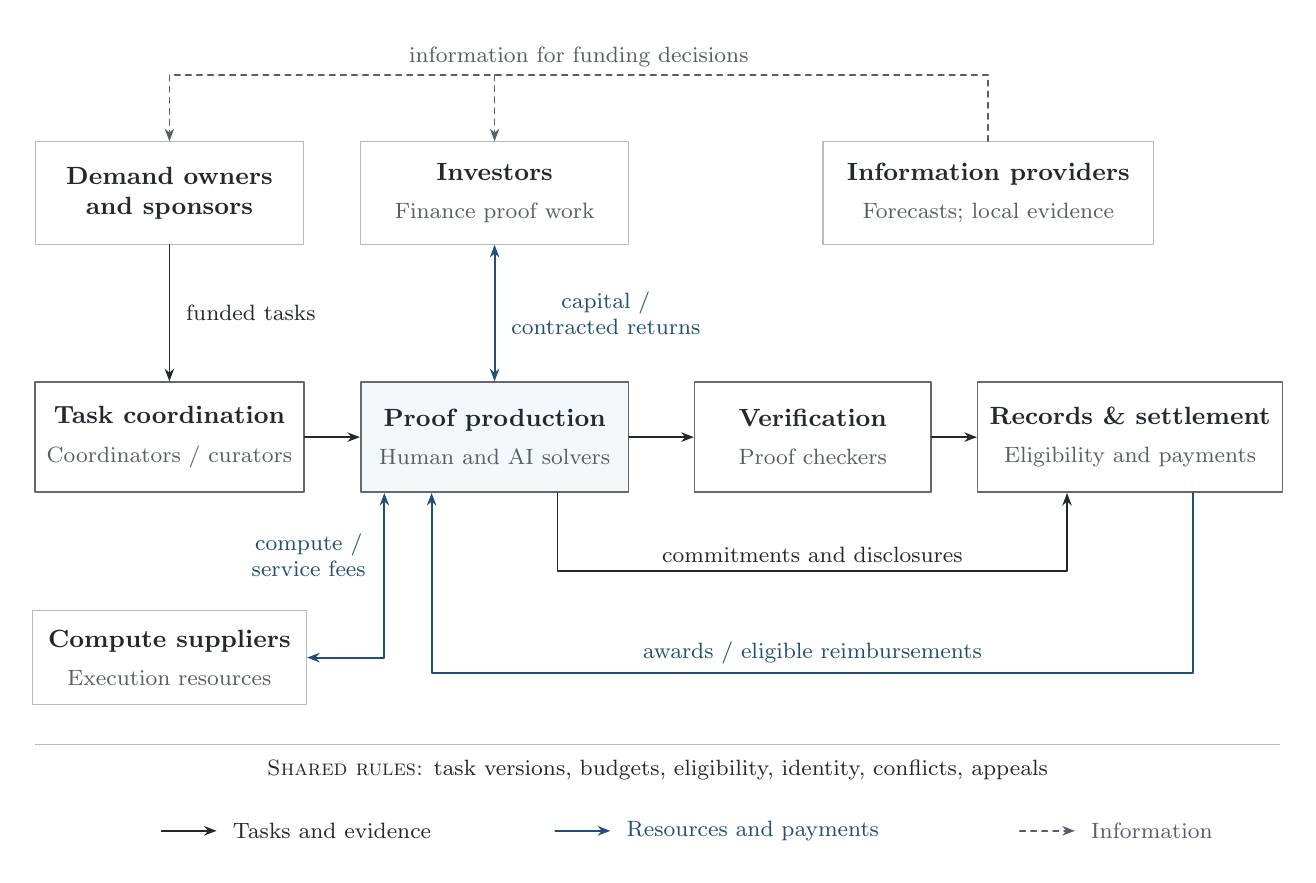
\begin{tikzpicture}[
  x=1mm,y=1mm,
  font=\fontsize{9}{11}\selectfont,
  text=ink,
  line cap=round,line join=round,
  >={Stealth[length=1.6mm,width=1.2mm]},
  core/.style={draw=ink!70,line width=.55pt,fill=white,
    minimum width=34mm,minimum height=14mm,inner sep=1.5mm,align=center},
  support/.style={draw=rule,line width=.45pt,fill=white,
    minimum height=13mm,inner sep=2mm,align=center},
  work/.style={->,draw=ink,line width=.65pt},
  resource/.style={draw=funding,line width=.7pt},
  information/.style={draw=muted,line width=.6pt,dash pattern=on 2pt off 2pt},
  label/.style={font=\fontsize{8}{9.5}\selectfont,inner sep=1mm,
    fill=white,align=center},
  legend/.style={font=\fontsize{8}{9.5}\selectfont,anchor=west,inner sep=0pt}
]
\path[use as bounding box] (0,-53) rectangle (160,52);

% The middle row is the principal flow of tasks and evidence.
\node[core] (tasks) at (18,0)
  {\textbf{Task coordination}\\[1mm]\detail{Coordinators / curators}};
\node[core,fill=pale] (solvers) at (59.3,0)
  {\textbf{Proof production}\\[1mm]\detail{Human and AI solvers}};
\node[core,minimum width=30mm] (checks) at (99.7,0)
  {\textbf{Verification}\\[1mm]\detail{Proof checkers}};
\node[core,minimum width=38mm] (records) at (140,0)
  {\textbf{Records \& settlement}\\[1mm]\detail{Eligibility and payments}};

\draw[work] (tasks.east) -- (solvers.west);
\draw[work] (solvers.east) -- (checks.west);
\draw[work] (checks.east) -- (records.west);

% Funding and information are inputs to the work, not stages of verification.
\node[support,minimum width=34mm] (sponsors) at (18,31)
  {\textbf{Demand owners}\\\textbf{and sponsors}};
\node[support,minimum width=34mm] (investors) at (59.3,31)
  {\textbf{Investors}\\[1mm]\detail{Finance proof work}};
\node[support,minimum width=42mm] (information) at (122,31)
  {\textbf{Information providers}\\[1mm]\detail{Forecasts; local evidence}};

\draw[work] (sponsors.south) -- node[label,right=1mm] {funded tasks} (tasks.north);
\draw[resource,<->] (investors.south) --
  node[label,right=1mm,text=funding] {capital /\\contracted returns} (solvers.north);
\draw[information,->] (information.north) -- (122,46) -- (18,46) -- (sponsors.north);
\draw[information,->] (59.3,46) -- (investors.north);
\node[label,text=muted,above] at (70,46) {information for funding decisions};

% Submission records and financial claims bypass the proof checker.
% Nested routes keep the two relations distinct and avoid crossings.
\draw[work] ($(solvers.south)+(8,0)$) -- (67.3,-17) --
  node[label,above=0mm] {commitments and disclosures} (132,-17) --
  ($(records.south)+(-8,0)$);
\draw[resource,->] ($(records.south)+(8,0)$) -- (148,-30) --
  node[label,above=0mm,text=funding] {awards / eligible reimbursements} (51.3,-30) --
  ($(solvers.south)+(-8,0)$);

\node[support,minimum width=34mm,minimum height=12mm] (compute) at (18,-28)
  {\textbf{Compute suppliers}\\[1mm]\detail{Execution resources}};
\draw[resource,<->] (compute.east) -- (45.3,-28) -- ($(solvers.south)+(-14,0)$);
\node[label,anchor=east,text=funding] at (44,-15) {compute /\\service fees};

% Governance constrains every relation; it is not another processing stage.
\draw[rule,line width=.45pt] (1,-39) -- (159,-39);
\node[font=\fontsize{8.5}{10}\selectfont,align=center,anchor=north,inner sep=0pt]
  at (80,-41) {\textsc{Shared rules:} task versions, budgets, eligibility, identity, conflicts, appeals};

\draw[work] (17,-50) -- (24,-50);
\node[legend] at (26,-50) {Tasks and evidence};
\draw[resource,->] (67,-50) -- (74,-50);
\node[legend,text=funding] at (76,-50) {Resources and payments};
\draw[information,->] (126,-50) -- (133,-50);
\node[legend,text=muted] at (135,-50) {Information};
\end{tikzpicture}
\end{document}
